\chapter{Introduction} \label{ch:intro}
\section{Motivation}
Occupancy estimation of a given space is an attractive use case of IoT (Internet of Things) devices. Knowing an approximate number of people may help by optimization of HVAC (Heating, Ventilation and Air-condition) consumption in a smart building. At home, a continuous monitoring of dwell time in each room may improve the safety of elder residents. Since the Corona pandemic breaks out, there has also been a strong demand for monitoring the people number inside a building for social distance controlling.

Many different sensors could be used to sense the number of people in a given space. \citeauthor{humansense2010survey} \cite{humansense2010survey} has classified the signals of human presenting into three categories and given their corresponding sensors. Static traits are the intrinsic attributes of a human, and are detectable even if the human stays still. Examples in this category are weight (measured by pressure sensor), reflectivity (camera) or emissivity (thermal sensor). Dynamic traits are the activities of a human, such as body movement detected by a ultrasonic sensor \cite{ultrasonic2012doorjamb} or speech detected by a microphone \cite{microphone}. Finally, external traits are the traits of objects carried by a person. A common case is a wearable RFID card \cite{RFID}. Due to the broad use of mobile phones nowadays, Wifi connection activity could also be a good indicator of human occupancy \cite{Wifi}. Beyond the three categories, a coarse estimation of a large amount of people could also be derived from the power consumption, number of lights switched on or the CO2 concentration in a building \cite{CO2}.

Among all sensors, the camera based method is chosen because its capability to detect human in both static/ dynamic scenarios, and the capability to handle complex scenarios with multiple human co-occurrence. An human count estimation by cameras could be obtained either by absolute counting or relative counting. The former method manages to overwatch the whole region of interest by one camera or by merging information from several cameras. The human count at a given time is determined by one single frame using object detection. Therefore, the counting algorithm is independent of camera frame rate as well as number of people entering/ leaving at the same time. The relative counting method only monitors the entrance of a room. The final count value is obtained by accumulating the number of entering/ exiting events. A tracking algorithm is required, therefore camera frame rate is critical. And for each frame, the tracking must be done strictly within the time window before the next frame is captured. Besides, when multiple people enter/ exit at the same time the algorithm should still be capable to track correctly.

Though absolute counting method may be effective for small rooms, a single camera cannot cover larger rooms. Our approach based on a relative counting method because we want to design a general device that is independent of the possible room space. Such a device is sometimes called a doorway turnstile \cite{griffiths2017empirical}.

However, how to monitor the people by a camera in a public space without intruding their privacy has poses a challenge to the device design. Due to concerns about privacy violation, RGB-cameras are usually excluded from home surveillance designs \cite{privacyconcerns}. Monitoring through a low-resolution infrared camera may solve the challenge fundamentally. The most remarkable feature of this kind of cameras is that they only have several pixels in vertical and horizontal directions respectively. Sometimes these cameras are referred as thermopile sensors. Thanks to the nature of low-resolution, a person could be detected but the identification of the person is impossible. Without the suspicion of leaking privacy, the monitor device is ideal for an application in public space, but also at home. Moreover, despite the fact that infrared cameras are usually much more expensive than common RGB-cameras, a low-resolution infrared camera is still affordable at the cost of low accuracy and scarce pixels, therefore it is suitable for mass deployment.
\section{Contribution}
This thesis proposes a human tracking algorithm which based on traditional CV (computer vision) methods of blob tracking. The algorithm takes top-view frame sequence of a infrared camera as input and outputs the relative count of the event. The absolute number of people in a room is obtained by accumulating the relative counts. A highlight of the algorithm is its capability to tracking multiple human instances, even when their blob representations merge or split. Several examples are shown in \autoref{fig:cornercases}.
\begin{figure}
  \centering
  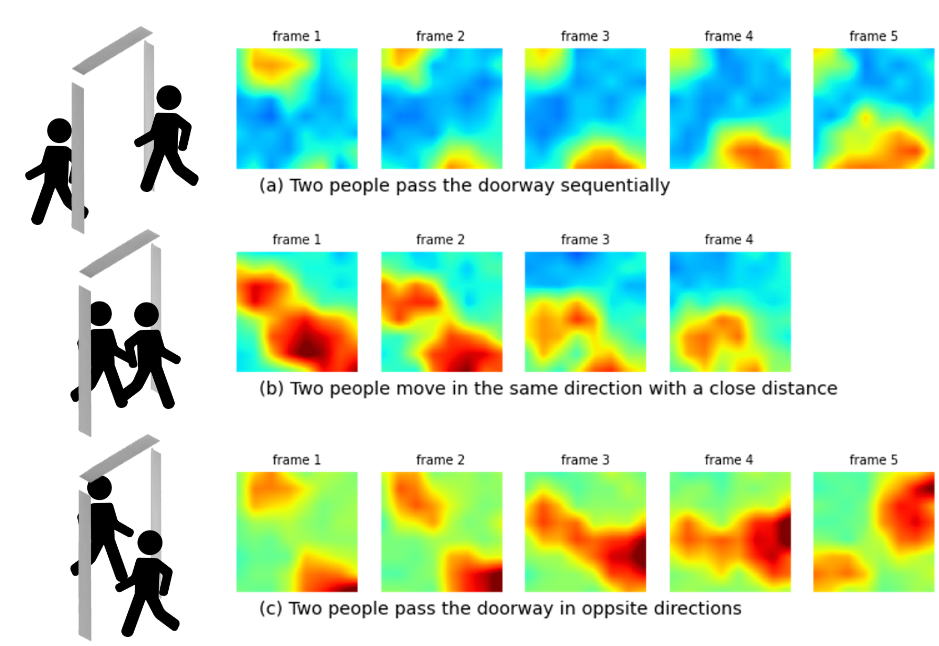
\includegraphics[width=0.85\textwidth]{figures/cornercases.PNG}
  \caption{several corner cases that the proposed algorithm is capable to handle}\label{fig:cornercases}
\end{figure}

\section{Thesis Overview}
In the next chapter, related works will be reviewed. In \autoref{ch:hardware}, objective of the design will be described in detail and certain choices of hardware is explained. In \autoref{ch:platform}, the communication protocol between the end node device and the data centralization platform is introduced. The main idea of the purposed algorithm is introduced in \autoref{ch:algorithm}. And \autoref{ch:evaluation} shows the final accuracy of the purposed algorithm based on a two-weeks in-situation test.







